% IEEE / BIBM double-blind draft.
\documentclass[conference]{IEEEtran}

\usepackage[T1]{fontenc}
\usepackage[utf8]{inputenc}
\usepackage{cite}
\usepackage{amsmath,amssymb}
\usepackage{graphicx}
\usepackage{booktabs}
\usepackage{array}
\usepackage{tikz}
\usepackage{url}

\usetikzlibrary{arrows.meta,positioning,fit,calc}

\newcommand{\methodname}{CrossEvidence}
\newcommand{\reconcile}{\texttt{context\_verifier\_reconcile}}
\newcommand{\hardrule}{\texttt{grounded\_hard\_rule}}
\newcommand{\sourcegrounded}{\texttt{source\_grounded\_reconcile}}
\newcommand{\deltext}{\ensuremath{\Delta}}

\title{\methodname: Citation-Valid Cross-Lingual Biomedical Evidence Reconciliation}

\author{}

\begin{document}
\maketitle

\begin{abstract}
Cross-lingual biomedical evidence extraction for clinical genetics requires both accurate structured fields and citations that can be audited against source literature. Direct LLM extraction can produce plausible values, but it does not guarantee that accepted evidence is grounded in recoverable source spans. We present \methodname{}, a citation-valid-by-construction evidence reconciliation framework for ACMG/ClinGen-style gene-disease evidence extraction. The method converts original-track and translated-track extraction candidates into a typed evidence graph, validates source spans, adds target-safe gene/disease context, and reconciles conflicts using verifier support, target specificity, cross-track agreement, and contradiction-aware scoring. We evaluate on a frozen $N=30$ ClinGen/ACMG-style benchmark against matched direct LLM, translate-then-extract, original-only, RAG-LLM, single-agent CoT, same-release-window citation-required frontier prompt-only, and grounded hard-rule baselines. Context-verifier reconciliation achieves $P=0.9205$, $R=0.9759$, and $F1=0.9474$, significantly improving over the grounded hard-rule baseline ($F1=0.8820$; $\deltext=+0.0654$; 95\% CI $=[0.0302, 0.1060]$; $p=0.0039$). It also exceeds the strongest same-window citation-required prompt-only frontier baseline, GPT-5, on raw $F1$ (0.9474 vs.\ 0.9222) and TraceableF1 (0.9474 vs.\ 0.9109). Accepted citations are recoverable from canonical source spans in the benchmark (CVR=1.0, HCR=0.0). Error analysis shows that the hardest remaining cases are relationship labels whose ClinGen validity semantics are not fully visible in article-local evidence.
\end{abstract}

\begin{IEEEkeywords}
biomedical information extraction, cross-lingual evidence, citation grounding, clinical genetics, ACMG, ClinGen
\end{IEEEkeywords}

\section{Introduction}
Clinical genetics evidence curation depends on structured, auditable facts rather than free-form summaries. A curator needs to know not only that an article mentions a gene and disease, but also which relationship is supported, where the evidence appears, and whether the cited passage can be inspected later. This requirement becomes more difficult in cross-lingual settings because evidence can be distorted by translation, lost during document conversion, or over-generalized by a language model that has no hard obligation to cite recoverable source spans.

Large language models provide a convenient interface for biomedical information extraction, but prompt-only systems often treat citations as generated text. This makes it difficult to distinguish a correct value supported by the source, a plausible value unsupported by the article, and a correct-looking citation that cannot be mapped back to the canonical document. For ACMG/ClinGen-style gene-disease evidence extraction, this is a methodological problem rather than only a product problem: the extraction method must make source validity and conflict resolution explicit enough to be measured.

We propose \methodname{}, a citation-valid-by-construction cross-lingual biomedical evidence reconciliation framework. The method extracts original-track and translated-track candidates, converts them into a typed evidence graph, verifies source spans, applies target-safe gene/disease context, and reconciles field conflicts with verifier support, target specificity, agreement, and contradiction penalties. The contribution is not the surrounding multi-agent software; it is the evidence-graph decision layer that turns citation validity into an acceptance invariant.

This paper makes five contributions:
\begin{itemize}
  \item a target-safe dual-track evidence graph for ACMG/ClinGen-style gene-disease evidence extraction;
  \item a context-verifier reconciliation method that combines source grounding, target specificity, cross-track agreement, and contradiction-aware scoring;
  \item traceability metrics that separate citation validity, hallucinated citation rate, span boundary quality, semantic support, and TraceableF1;
  \item a frozen $N=30$ evaluation against matched LLM baselines and grounded internal ablations, with paired statistics and explicit limitations;
  \item a citation-required prompt-only frontier model sweep using a same-release-window cohort and a single OpenAI-compatible provider gateway, isolating method value from prompt engineering alone.
\end{itemize}

\section{Related Work}
Biomedical information extraction systems have long addressed named entity recognition, relation extraction, and entity normalization for genes, diseases, variants, and clinical findings. Recent reviews show that clinical LLM evaluation still splits into knowledge-based benchmarks and practice-oriented tasks, and the resulting performance gap is non-trivial \cite{gong2025knowledgepractice,chen2026operationalizing}.

Cross-lingual biomedical IE is commonly handled through translate-then-extract pipelines or multilingual model prompting. These approaches can improve coverage, but they also introduce semantic drift and make it harder to determine whether a final structured value came from the original source, the translation, or an arbitration step \cite{li2025framefirst,guillen2026mapcare}.

LLM and RAG systems add another layer: they can retrieve documents and produce fluent answers with citations, but the citation itself may still be generated rather than programmatically validated. \methodname{} differs by making accepted evidence depend on recoverable source spans and by exposing citation validity as a quantitative metric \cite{pandit2025medhallu,onweller2026cited}.

Clinical genetics curation adds domain-specific constraints. Gene-disease relationships can encode external validity judgments, and article-local evidence may not fully express a final ClinGen label. For this reason, our method separates source-visible extraction errors from source-label visibility limits and avoids using gold ClinGen labels as runtime inputs \cite{queen2025cgbench,mortezaagha2026schemaconstrained,birgmeier2020avada,richards2015acmg,riggs2020cnv,brnich2020ps3bs3,tavtigian2018bayesian,aboutayoun2018pvs1}.

\section{Task and Dataset}
The task is to extract structured evidence fields from biomedical literature for a target gene-disease context. The current frozen benchmark emphasizes three fields: \texttt{A.gene\_symbol}, \texttt{B.disease\_diagnosis}, and \texttt{A.gene\_disease\_relationship}. Each accepted evidence item must include a source span that can be audited against canonical document text.

We evaluate on a frozen ClinGen/ACMG-style benchmark with 30 entries. The benchmark package has 30/30 Phase 2 artifacts covered and no remaining pipeline gaps. Runtime inputs are restricted to source article text and metadata, runtime extraction artifacts, target-safe ontology/context metadata, and programmatically verified source spans. The method does not use expected fields, ClinGen classification labels, evaluator matches, or gold relationship labels at runtime.

Table~\ref{tab:dataset} summarizes the frozen dataset and reproducibility anchor.

\begin{table*}[t]
\centering
\caption{Dataset composition and reproducibility anchor.}
\label{tab:dataset}
\setlength{\tabcolsep}{4pt}
\renewcommand{\arraystretch}{1.08}
\footnotesize
\begin{tabular}{lccccc}
\toprule
total\_entries & covered\_count & needs\_pipeline\_count & frozen\_entry\_count & git\_commit & ablation\_report \\
\midrule
30 & 30 & 0 & 30 & 7d13b1a8206476cd8c0e750684f53d6dc80b5c55 & \texttt{reconcile\_ablation\_20260615\_010725.json} \\
\bottomrule
\end{tabular}
\end{table*}

\section{Method}
\subsection{Dual-Track Candidate Generation}
\methodname{} first extracts candidate evidence from two tracks: the source/original track and a translated track. The two tracks are not treated as independent final answers. Instead, their outputs become candidates in a shared evidence graph. This design allows the method to compare semantically similar values, identify disagreements, and preserve the source span supporting each candidate.

\subsection{Evidence Graph}
The evidence graph contains target gene nodes, target disease nodes, evidence field nodes, candidate value nodes, source span nodes, track nodes, and document block nodes. Edges connect candidates to fields, tracks, source spans, target-gene support, target-disease support, equivalent values, and contradictory values. This graph is the formal object used for reconciliation.

Each candidate contains:
\begin{equation}
\begin{aligned}
(\text{entry\_id}, \text{field\_id}, \text{raw\_value}, \text{normalized\_value}, \text{track}, \text{block\_id}, \text{span\_id},\\
\text{source\_score}, \text{model\_confidence}, \text{target\_gene\_match}, \text{target\_disease\_match},\\
\text{verifier\_support}, \text{contradiction\_penalty}, \text{source\_validity})
\end{aligned}\end{equation}

\subsection{Citation-Valid Acceptance}
A candidate can only be accepted when at least one supporting source span is recoverable from canonical source text. The method prefers span id, page, and offset validation where available, and falls back to normalized source text matching when necessary. LLM output is not allowed to invent a citation string; accepted citations are emitted from verified span metadata.

\subsection{Target-Safe Context}
Target-safe context adds known gene and disease aliases, ontology metadata, and source-observed disease aliases when they are present in the article and compatible with the target. This improves disease boundary selection without using benchmark answer keys or ClinGen classification labels. The context layer is intentionally conservative: article-local symptom terms or broad unrelated ontology terms are not promoted to target aliases.

\subsection{Context-Verifier Reconciliation}
For each field and normalized candidate value, \methodname{} computes a reconciliation score:
\begin{equation}
\begin{aligned}
\text{score} =\;& w_{\text{source}} \cdot \text{source\_score}
 + w_{\text{agree}} \cdot \text{cross\_track\_agreement}
 + w_{\text{support}} \cdot \text{verifier\_support} \\
& + w_{\text{target}} \cdot \text{target\_specificity}
 + w_{\text{conf}} \cdot \text{extractor\_confidence}
 + w_{\text{status}} \cdot \text{status\_score}
 - w_{\text{contra}} \cdot \text{contradiction\_penalty}
\end{aligned}\end{equation}

The accepted field value is the best-scoring value that satisfies source validity, verifier support, target specificity, and contradiction checks. If source support is weak or the best value is not sufficiently separated from alternatives, the method can abstain or mark the conflict for review rather than accepting an unsupported value.

\begin{figure*}[t]
\centering
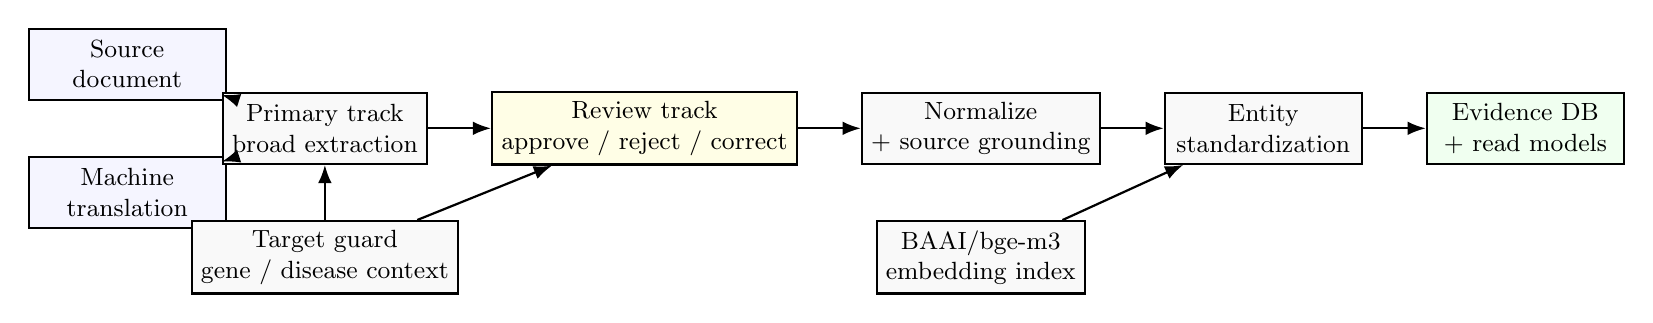
\begin{tikzpicture}[
  font=\small,
  node distance=7mm and 8mm,
  block/.style={draw=black, thick, rectangle, minimum height=9mm, minimum width=25mm, align=center, fill=gray!5},
  input/.style={draw=black, thick, rectangle, minimum height=9mm, minimum width=25mm, align=center, fill=blue!4},
  review/.style={draw=black, thick, rectangle, minimum height=9mm, minimum width=25mm, align=center, fill=yellow!10},
  output/.style={draw=black, thick, rectangle, minimum height=9mm, minimum width=25mm, align=center, fill=green!6},
  edge/.style={-Latex, thick}
]
  \node[input] (source) {Source\\document};
  \node[input, below=of source] (translation) {Machine\\translation};
  \node[block, right=12mm of $(source)!0.5!(translation)$] (primary) {Primary track\\broad extraction};
  \node[review, right=of primary] (reviewer) {Review track\\approve / reject / correct};
  \node[block, right=of reviewer] (ground) {Normalize\\+ source grounding};
  \node[block, right=of ground] (entities) {Entity\\standardization};
  \node[output, right=of entities] (readmodel) {Evidence DB\\+ read models};

  \node[block, below=of primary] (target) {Target guard\\gene / disease context};
  \node[block, below=of ground] (embedding) {BAAI/bge-m3\\embedding index};

  \draw[edge] (source) -- (primary);
  \draw[edge] (translation) -- (primary);
  \draw[edge] (primary) -- (reviewer);
  \draw[edge] (reviewer) -- (ground);
  \draw[edge] (ground) -- (entities);
  \draw[edge] (entities) -- (readmodel);
  \draw[edge] (target) -- (primary);
  \draw[edge] (target) -- (reviewer);
  \draw[edge] (embedding) -- (entities);
\end{tikzpicture}

\caption{CrossEvidence pipeline. Original and translated tracks generate candidates that are fused into a typed evidence graph, filtered by source-span validity, and reconciled by a verifier-aware scoring policy before accepted evidence is emitted with recoverable citations.}
\label{fig:pipeline}
\end{figure*}

\section{Evaluation Design}
We compare the proposed \reconcile{} method with five matched extraction baselines and one grounded internal baseline:
\begin{itemize}
  \item B0: direct LLM extraction;
  \item B1: translate then extract;
  \item B2: original-only extraction;
  \item B3: keyword RAG + LLM;
  \item B4: single-agent CoT;
  \item B5: grounded hard-rule internal baseline;
  \item B6-B10: citation-required prompt-only frontier sweep.
\end{itemize}

All B0-B4 baseline reports are matched to the same 30 benchmark entries as the system. We report precision, recall, F1, paired bootstrap confidence intervals, and paired sign-test $p$-values. We also report traceability metrics:
\begin{itemize}
  \item Citation Validity Rate (CVR): accepted cited spans recoverable from canonical source text;
  \item Hallucinated Citation Rate (HCR): accepted citations not mappable to canonical source text;
  \item Span Boundary F1: token overlap between predicted and reference/support span text;
  \item Evidence Support Rate (ESR): fraction of accepted evidence semantically supported by the source according to the verifier/evaluation audit;
  \item TraceableF1: extraction F1 constrained by citation validity;
  \item Cross-Lingual Consistency (CLC): agreement between original and translated tracks before final arbitration.
\end{itemize}

B0-B4 provide matched extraction baselines but do not expose comparable citation surfaces in the current reports. B6-B10 use the same citation-required JSON prompt, the same input window, the same integrated OpenAI-compatible provider gateway, and model aliases from a comparable release window: GPT-5 (2025-08-07), DeepSeek V3.1 (2025-08-21), Qwen3-Max (2025-09-23), Claude Sonnet 4.5 (2025-09-29), and GLM-4.6 (2025-09-30). Therefore, B6-B10 can be compared on CVR/HCR/TraceableF1, while B0-B4 are retained for the established extraction-quality ladder.

\section{Results}
\subsection{Main Comparison}
Table~\ref{tab:main} shows the main matched comparison. The proposed method achieves F1=0.9474 on the frozen $N=30$ benchmark. It significantly improves over the grounded hard-rule internal baseline, and it remains competitive with the strongest matched LLM baseline.

\begin{table*}[t]
\centering
\caption{Main method versus matched baselines.}
\label{tab:main}
\setlength{\tabcolsep}{3.5pt}
\renewcommand{\arraystretch}{1.08}
\footnotesize
\begin{tabular}{lcccccc}
\toprule
method & role & precision & recall & F1 & $\Delta$F1 vs.\ \hardrule & sign-test $p$ \\
\midrule
B0 & baseline & 0.9398 & 0.9176 & 0.9286 &  &  \\
B1 & baseline & 0.9136 & 0.8916 & 0.9024 &  &  \\
B2 & baseline & 0.9125 & 0.8795 & 0.8957 &  &  \\
B3 & baseline & 0.9367 & 0.8706 & 0.9024 &  &  \\
B4 & baseline & 0.9277 & 0.9167 & 0.9222 &  &  \\
\reconcile{} & ours & 0.9205 & 0.9759 & 0.9474 & 0.0654 & 0.0039 \\
\bottomrule
\end{tabular}
\end{table*}

The paired statistics against \hardrule{} show $\Delta F1=+0.0654$, 95\% CI $=[0.0302, 0.1060]$, and sign-test $p=0.0039$. The candidate exceeds the strongest matched LLM baseline B0 by +0.0188 F1, but this does not meet the pre-declared +0.03 strong-superiority threshold. We therefore frame the result as traceability-centered competitive extraction with significant improvement over the grounded internal baseline, not as broad superiority over all LLM baselines.

\subsection{Ablation}
Table~\ref{tab:ablation} shows that context-verifier reconciliation provides the strongest F1 among the internal variants.

\begin{table}[t]
\centering
\caption{Ablation study.}
\label{tab:ablation}
\setlength{\tabcolsep}{4pt}
\renewcommand{\arraystretch}{1.08}
\small
\begin{tabular}{lcccc}
\toprule
strategy & total & precision & recall & F1 \\
\midrule
dual\_union & 30 & 0.7935 & 0.9733 & 0.8743 \\
\hardrule{} & 30 & 0.8068 & 0.9726 & 0.8820 \\
\sourcegrounded{} & 30 & 0.8182 & 0.9730 & 0.8889 \\
\reconcile{} & 30 & 0.9205 & 0.9759 & 0.9474 \\
\bottomrule
\end{tabular}
\end{table}

The field-level results show that gene symbol extraction is strongest (F1=0.9831), disease diagnosis is also strong (F1=0.9655), and gene-disease relationship remains the hardest field (F1=0.8889).

\subsection{Traceability}
Table~\ref{tab:traceability} reports traceability metrics for the candidate.

\begin{table}[t]
\centering
\caption{Traceability metrics.}
\label{tab:traceability}
\setlength{\tabcolsep}{4pt}
\renewcommand{\arraystretch}{1.08}
\small
\begin{tabular}{lcccccc}
\toprule
strategy & CVR & HCR & SpanBoundaryF1 & ESR & TraceableF1 & CLC \\
\midrule
\reconcile{} & 1.0 & 0.0 & 0.7467 & 0.9205 & 0.9474 & 0.194 \\
\bottomrule
\end{tabular}
\end{table}

The candidate has CVR=1.0 and HCR=0.0 over 88 accepted citations in the frozen benchmark. This supports the citation-valid-by-construction claim for accepted evidence in this evaluation. It does not imply semantic perfection: ESR is 0.9205, and the remaining errors are analyzed separately.

Internal grounded traceability baselines are lower in TraceableF1: \hardrule{} reaches 0.8820 and \sourcegrounded{} reaches 0.8889. B0-B4 do not currently expose citation surfaces, so direct HCR comparisons against those baselines require future citation-generating baseline runs. The citation-required B6-B10 prompt-only sweep below provides the direct prompt-only traceability comparison.

\subsection{Same-Window Prompt-Only Frontier Sweep}
To separate model strength from method design, we additionally evaluate citation-required prompt-only baselines across five mainstream model families released within a comparable 2025 frontier window. These baselines differ only by the provider model alias recorded in the manifest; they use the same prompt mode, temperature, input window, raw OpenAI-compatible call path, and evaluation logic.

\begin{table*}[t]
\centering
\caption{Citation-required prompt-only frontier sweep.}
\label{tab:prompt-sweep}
\setlength{\tabcolsep}{3pt}
\renewcommand{\arraystretch}{1.05}
\scriptsize
\begin{tabular}{llccccc}
\toprule
baseline & model & release & F1 & CVR & HCR & TraceableF1 \\
\midrule
B6\_GPT5\_PROMPT\_CITE & gpt-5-2025-08-07 & 2025-08-07 & 0.9222 & 0.9878 & 0.0122 & 0.9109 \\
B7\_DEEPSEEK\_V31\_PROMPT\_CITE & deepseek-v3.1 & 2025-08-21 & 0.6765 & 0.7200 & 0.2800 & 0.4871 \\
B8\_QWEN3\_MAX\_PROMPT\_CITE & qwen3-max & 2025-09-23 & 0.8535 & 0.8356 & 0.1644 & 0.7132 \\
B9\_CLAUDE\_SONNET45\_PROMPT\_CITE & claude-sonnet-4-5-20250929 & 2025-09-29 & 0.8820 & 0.7342 & 0.2658 & 0.6476 \\
B10\_GLM46\_PROMPT\_CITE & glm-4.6 & 2025-09-30 & 0.7143 & 0.6724 & 0.3276 & 0.4803 \\
\bottomrule
\end{tabular}
\end{table*}

The strongest prompt-only frontier baseline is GPT-5, with F1=0.9222 and TraceableF1=0.9109. \methodname{} remains higher on both raw F1 and TraceableF1 in this frozen comparison. We do not claim paired statistical superiority over each frontier model unless such tests are added; the result is used to show that prompt engineering alone does not close the traceable-extraction gap in this benchmark.

\subsection{Error Analysis}
Table~\ref{tab:error} summarizes remaining errors.

\begin{table}[t]
\centering
\caption{Error breakdown.}
\label{tab:error}
\setlength{\tabcolsep}{4pt}
\renewcommand{\arraystretch}{1.08}
\small
\begin{tabular}{lcc}
\toprule
root\_cause & error\_count & strategy \\
\midrule
source\_label\_visibility\_limit & 5 & \reconcile{} \\
disease\_boundary\_error & 2 & \reconcile{} \\
candidate\_absent & 2 & \reconcile{} \\
\bottomrule
\end{tabular}
\end{table}

The dominant remaining issue is not a simple extraction failure. Five relationship mismatches are classified as source-label visibility limits: the article-local evidence expresses weak association, prediction, or partial support, while the benchmark label reflects external ClinGen validity semantics. We keep these cases separate to avoid leaking gold curation labels into runtime extraction.

\section{Discussion and Limitations}
The results support a conservative Main Paper claim. \methodname{} significantly improves over a grounded hard-rule internal baseline and remains competitive with matched LLM baselines while adding deterministic citation-valid acceptance. The method is strongest when the evidence needed for a field is visible in the article and can be linked to target-safe gene/disease context.

The study has several limitations. First, the frozen benchmark contains 30 ClinGen/ACMG-style entries. This is suitable for controlled method analysis and paired statistics, but not for broad claims of general biomedical IE superiority. Second, the candidate's margin over the strongest matched B0-B4 LLM extraction baseline is +0.0188 F1, below the pre-declared +0.03 strong-superiority threshold. Third, the B6-B10 prompt-only frontier sweep is tied to exact provider aliases and a same-release-window cohort; hosted model behavior and routing may change over time, so the manifest is part of the frozen evidence package. Fourth, some gene-disease relationship labels reflect external ClinGen validity curation not fully visible in article-local evidence. Finally, \methodname{} extracts, grounds, and reconciles evidence fields for expert review; it is not an autonomous clinical decision-support or ACMG classification system.

Future work should expand the benchmark, add citation-generating direct LLM and RAG baselines for direct HCR comparison, and build a native multilingual biomedical genetics gold set. Curated ClinGen context could also be tested as a separate external-knowledge ablation, but it should not be mixed into source-only extraction without disclosure.

\section{Conclusion}
\methodname{} frames cross-lingual biomedical evidence extraction as traceability-constrained evidence reconciliation rather than prompt-only generation. On a frozen ACMG/ClinGen-style benchmark, context-verifier reconciliation significantly improves over a grounded internal baseline, remains competitive with matched LLM baselines, and enforces citation-valid-by-construction accepted evidence. The current evidence supports a conservative Main Paper submission centered on auditable, source-grounded cross-lingual biomedical IE.

\bibliographystyle{IEEEtran}
\bibliography{refs}

\end{document}
